\section{Dokumentation der Arbeitsweise}

Die Phase der Qualitätssicherung wurde genutzt, um das in der Implementierungsphase angefertigte Softwareprodukt zu verbessern. Es wurden Anstrengungen unternommen, Fehler zu erkennen und zu beheben sowie die Robustheit und Benutzerfreundlichkeit des Programms zu erhöhen.
Zudem konnten einige offene Aufgaben der Implementierungsphase gelöst werden.

\subsection{Tools}

\begin{itemize}
\item Git/GitHub: Versionskontrolle
\item Continuous Integration (Travis CI): Open-Source-Software für kontinuierliche Integration
\item IntelliJ: Entwicklungsumgebung
\item JUnit: Framework zum Testen von Java-Programmen
\end{itemize}

\subsection{Vorgehen}

Die Klassen der Pakete Model und Controller wurden mittels Modultests über das Framework JUnit getestet. Hierzu wurden für sie jeweils eine eigene Testklasse erstellt. Diese bestehen aus einer Vielzahl von Testfällen, die jeweils ausgewiesene Funktionalität auf Richtigkeit prüfen.

Aufgrund des naturgemäß hohen Grades an Benutzerinteraktion im Paket View, waren an dieser Stelle Modultests nicht zielführend. Stattdessen wurde das Programm vom QA-Team manuell auf Fehler untersucht, indem zum einen naheliegende Anwendungsfälle durchgespielt wurden, zum anderen aber auch versucht wurde, Fehlverhalten, das durch ungewöhnliches Nutzerverhalten hervorgerufen werden könnte, offenzulegen.

Hat ein Teammitglied einen Fehler entdeckt, so wurde dieser auf der Plattform GitHub als sog. Issue festgehalten. Diesem Issue wurde anschließend ein Zuständiger zugeteilt. Sobald der Zuständige das Problem beheben konnte, wurde der Issue geschlossen.\\
Die hierfür notwendigen Änderungen am Programm wurden auf einem neuen Entwicklungszweig vorgenommen. Durch Travis-CI wurde dabei sichergestellt, dass auch nach den Änderungen alle Testfälle erfolgreich durchlaufen werden. Vor dem Verschmelzen mit dem Hauptzweig wurde die Änderung von mindestens einem weiteren Teammitglied gesichtet (Code-Review).

\begin{figure}[H]
	\centering
	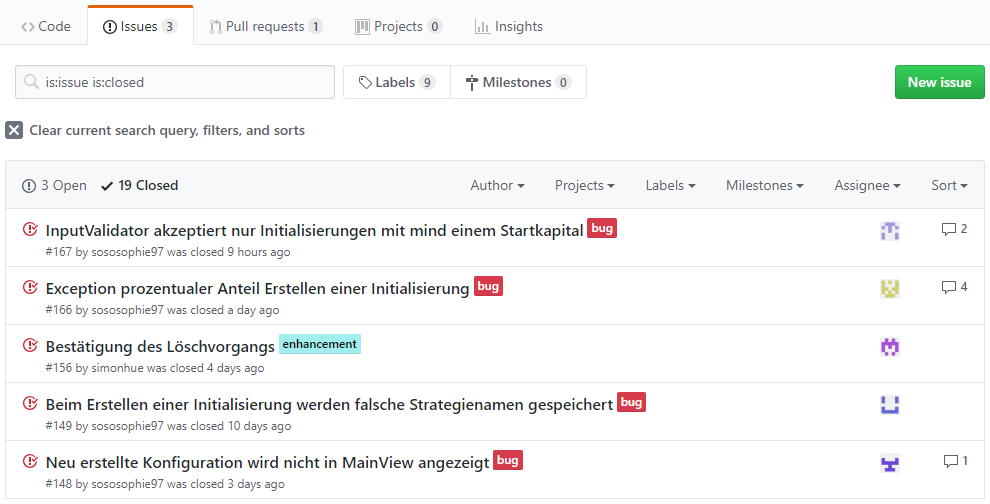
\includegraphics[width=1.1\textwidth]{qs_1.png}
	\caption{Übersicht der neusten geschlossenen Issues auf GitHub}
\end{figure}